\chapter{Esplorazione di un grafo anonimo}

\emph{D. Ilcinkas -
    Setting Port Number For Fast Graph Exploration}\\

Affrontiamo adesso il seguente problema: \textbf{Vogliamo inserire dei numeri di
    porta in modo tale che un robot esplori sequenzialmente un grafo in modo
    periodico (cioè ricominci quando ha finito) utilizzando il percorso minimo.}

%e vogliamo che ci metta meno tempo possibile, ovvero che il percorso sia minimo.}

Specifichiamo il robot come un'\textbf{automa di Mealy}.

Il grafo in input ha topologia incognita ed il robot ha \textbf{orientamento
    locale} ovvero le etichette sugli archi uscenti dal nodo $v$ sono distinti e con
valori:
\begin{center}
    $1, \cdots, d_v = \deg (v)$\end{center}
\begin{center}
    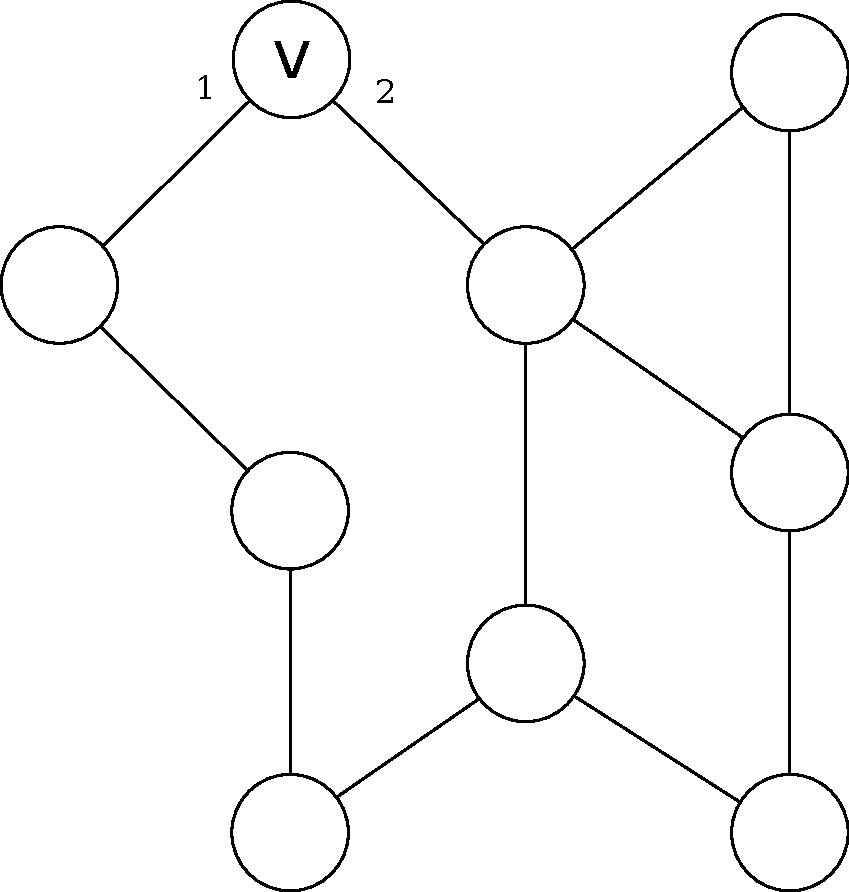
\includegraphics[scale=0.3]{capitoli/esplorazione-grafo-anonimo/imgs/n_25}
\end{center}

Per il robot dobbiamo specificare la \textbf{funzione di transizione}:\\\\
\begin{center}
    $f(s,i,d_v) = (s',i')$
\end{center}

Dove:
\begin{itemize}
    \item $s$ = stato in cui sono;
          %\item $i$ = porta in cui esco.
    \item $i$ = porta in cui entro nel nodo $v$ in cui vado.
    \item $d_v = \deg(v)$ Grado del nodo in cui arrivo.
    \item $s'$ = stato in cui vado una volta entrato in $v$;
    \item $i'$ = porta in cui esco quando sono su $v$.
\end{itemize}

La scelta migliore sarebbe trovare uno Spanning Tree del grafo incognito che
stiamo considerando, in questo caso la lunghezza ($\Pi$) sarebbe $\Pi(n) =
    2(n-1)$ dove:
\begin{itemize}
    \item 2 indica il dover scendere e risalire il grafo (stiamo attuando una DFS)
    \item $n-1$ indica il numero dei nodi dell'albero
\end{itemize}
\textbf{Perché il lower bound del problema è $n$?}\\
Il LowerBound del problema dovrebbe essere esattamente $\Omega(n)$ e non $2n$,
ovvero si devono necessariamente attraversare tutti i nodi. Troviamo un percorso
di lunghezza $\Pi$ pari ad $n$ su un Anello, per esempio, o se esiste nel grafo
considerato un sottografo che è un anello, per poi etichettarlo in maniera tale
da entrare sempre da porta 1 ed uscire sempre da porta 2. Il problema è che non
sono sicuro che questo ciclo esista sempre. I grafi in cui è presente un ciclo
di questo tipo al loro interno sono detti Hemiltoniani, ma sapere se un grafo è
Hemiltoniano è un problema NP-completo. Ovvero:\\ Dato un grafo $G$ trovare un
sotto ciclo che tocchi tutti i nodi del grafo $G$ passando solamente una volta per
ogni arco e che ritorni al nodo di partenza.\\
Dato che questa strada è complessa scelgo di costruire prima uno Spanning Tree
del grafo e poi far muovere l'automa li dentro, anche se passa più volte per
arco. \\\textbf{Un esempio di un grafo che non ammette ciclo hemiltoniano è un
    qualsiasi grafo avente almeno un nodo con grado uno.} Poiché arrivati in quel
nodo si deve necessariamente tornare indietro e quindi passare per un arco due
volte. Dato che si vuole costruire uno Spanning Tree, ci sarà necessariamente un
nodo di grado uno. Quindi è necessario tenere $2(n-1)$ come lowerBound e non
$n$.

\subsection*{Risultato di impossibilità}
Non è possibile risolvere il problema di esplorazione periodica di un grafo se i
numeri di porta sono dati arbitrariamente (se i numeri di porta sono specificati
da un avversario, è facile far entrare l'automa in loop).

Nel 2006 Dobrev ha dato un upper bound al problema, pari a $10n$, usando la
\textbf{regola della mano destra} ed usando \textbf{automa ad oblio} (non
cambiano stato e ne ha solo uno):
\begin{center}
    $f(s,i,d) = (s,(i~mod~d) + 1)$
\end{center}
L'automa quindi uscirà su porta 1 quando la i è pari al grado ($d$) del nodo.

\section{Come possiamo migliorare il bound di 10n?}
%Abbiamo esplorato tutti i nodi ed il robot torna nel nodo di partenza, uscendo
%dalla porta di partenza. Nel nostro caso 
Consideriamo che l'automa abbia \textbf{memoria finita} nella quale non sono
memorizzati i numeri di porta, poiché in un grafo qualsiasi non conosciamo il
deg massimo.

Il periodo trovato è:
\begin{center}
    $\pi(n) \leq 4n-2$
\end{center}
Per questo miglioramento sono necessari 3 stati, aggiungere stati equivale ad
aggiungere memoria all'automa. L'obiettivo è quello di costruire uno spanning
tree in modo da risparmiare la visita di alcuni archi inserendo opportunamente i
numeri di porta. \\
Fondamentale il fatto che posizioneremo dei numeri di porta in maniera tale che
se esco da porta $i$ e quell'arco non è appartenente allo Spanning Tree, allora
nessun altro arco con porta maggiore di $i$ sarà appartenente allo spanning
tree. Questo è utilizzato dall'automa per evitare di testare troppi archi
durante l'attraversamento.

\section{ST con Orientamento Locale:}
Consideriamo un generico spanning tree di $G$, chiamato $T$.
\begin{itemize}
    \item Sia $F \subseteq E$ il sottoinsieme di archi appartenenti all'albero
          $T$.
    \item $\forall v \in V$, $F_v$ denota l'insieme degli archi incidenti a $v$ in
          $T$.
\end{itemize}

\begin{definition}\label{def:st-locorient}
    Un \textbf{orientamento locale} degli archi di un grafo è detto
    \textbf{compatibile} con un ST $T=(V,F)$ se e solo se:
    \begin{enumerate}
        \item $\forall e \in E$, almeno uno dei suoi numeri di porta è 1 se e solo
              se $e \in F$;
        \item $\forall v \in V$ gli archi appartenenti allo ST ($F_v$) hanno i loro
              numeri di porta da 1 a $|F_v|$.
    \end{enumerate}
\end{definition}

\textbf{Prima di poter far girare l'automa su un grafo,
    bisogna sia costruire uno spanning tree sia definire un orientamento locale.
    L'algoritmo Small-Ports permette di fare entrambe le cose insieme.}

\section{Algoritmo Small-Ports per la costruzione dello ST con orientamento locale}
Questo algoritmo permette di costruire un orientamento locale dato in input uno
Spanning Tree, che permetterà al Robot di poter risolvere il problema proposto
ad inizio capitolo.
\begin{enumerate}
    \item Come input si ha uno Spanning Tree $T$ di un grafo generico $G$. Sia $r$
          la sua radice.

    \item $\forall v \neq r$, assegna la porta 1 all'arco di $T$ che conduce ad
          $r$. In $r$, assegna 1 ad un qualunque (quindi scelto arbitrariamente) arco in
          $F_r$.
    \item $\forall v$, assegna arbitrariamente le porte da 2 a $|F_v|$ (che indica
          da 2 al grado del nodo $v$) ai rimanenti archi $F_v$ (appartenenti a T quindi)
          se esistono.
    \item Infine $\forall v$, assegna arbitrariamente i numeri di porta da
          $|F_v|+1$ a $d_v$, agli archi a cui non sono ancora stati assegnati dei numeri
          di porta, se esistono.
\end{enumerate}

\textbf{Spiegazione dei punti precedenti a parole:} I primi due punti sono
intuitivi, il terzo invece fa sempre riferimento al fatto che vanno assegnati i
numeri di porta più piccoli agli archi dove nell'altra estremità c'è porta 1,
ovvero archi sempre appartenenti allo ST. Il quarto si riferisce all'inserimento
dei numeri di porta di tutti gli archi che nell'altra estremità non hanno porta
1 e quindi non sono appartenenti allo ST.

Date queste regole quindi, qualora si uscisse da una porta con etichetta 1
allora siamo sicuri che si è attraversato un arco appartenente allo ST. Se così
fosse però molto probabilmente (a meno che il nodo su cui andiamo non abbia
cardinalità = 1) non avrà anch'esso porta 1, e quindi bisognerà testare quale
dei suoi archi uscenti è quello appartenente allo ST.
\newpage
\example{
    \begin{center}
        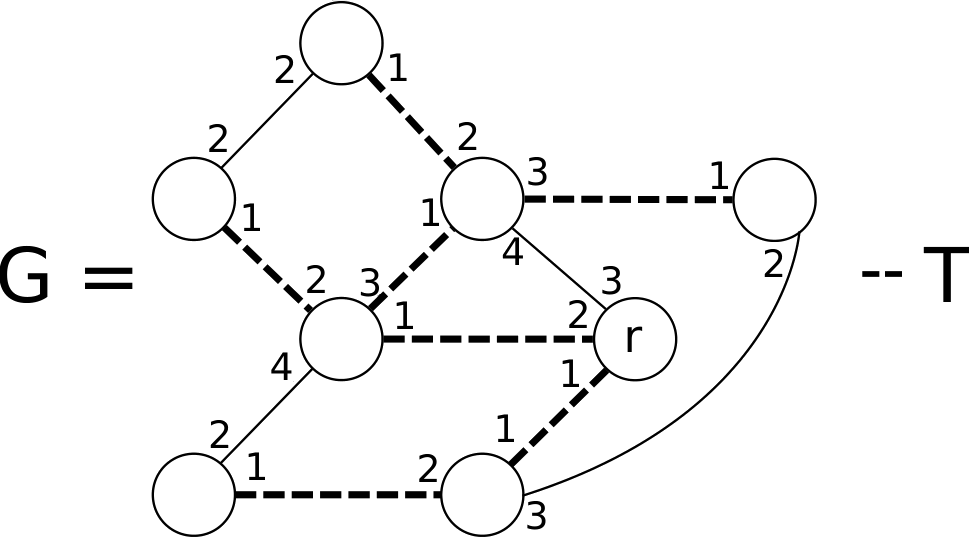
\includegraphics[scale=1.0]{capitoli/esplorazione-grafo-anonimo/imgs/n_26.png}
    \end{center}
}

È un orientamento locale in quanto $\forall v \in V$ tutte le etichette vanno da
1 a $d_v$.

È compatibile con $T$ poiché valgono \textit{1.} e \textit{2.}
(\ref{def:st-locorient}).

Otteniamo quindi uno e un solo arco con etichette entrambe 1, il quale non ci
consente di dire quale dei due nodi estremi è la radice. Abbiamo ottenuto quindi
uno Spanning Tree con orientamento locale. Andiamo a definire come si dovrà
muovere l'automa su di questo.
%\subsection*{Complessità} \begin{itemize} \item Passo 1: $=(m \log n)$ \item
%Passo 2: $O(n)$ \item Passo 3 + Passo 4: $2m -n$ \end{itemize} Quindi la
%complessità totale è di $m \log n + 2m$.

\section{Funzione di transizione}
Trovato lo Spanning Tree del nostro grafo di partenza attraverso il corretto
inserimento dei numeri di porta, analizziamo i movimenti del robot. Esso si basa
su tre stati:
\begin{itemize}
    \item \textit{Normal}, l'automa sta percorrendo per certo un arco in $T$
    \item \textit{Test}, percorre un arco che può o meno essere in $T$
    \item \textit{Backtrack}, percorre un arco che sicuramente non è in $T$
\end{itemize}
\subsection{N: Normal}
\begin{center}
    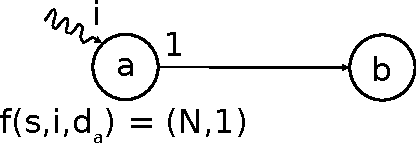
\includegraphics[scale=0.7]{capitoli/esplorazione-grafo-anonimo/imgs/n_27}
\end{center}
%Per la regola numero 2 definita precedentemente (quella dell'inserire etichetta
%1 sempre nell'arco che va verso la radice), se esco da $a$ su porta 1, allora
%$b$ è il mio padre nello ST, quindi il robot esce in stato $N$, in quanto
%quell'arco è sicuramente appartenente allo ST. Abbiamo che \textbf{d} = Grado
%del nodo corrente e \textbf{i} = Porta d'ingresso.
\begin{equation}
    f(N,i,d) =
    \left\{
    \begin{array}{r
            @{\quad{\mbox{se}}\quad}
            l}
        (N,1)   & i = d    \\
        (T,i+1) & i \neq d \\
    \end{array}
    \right.
\end{equation}

\begin{itemize}
    \item Se la porta in cui entro su $v$ è esattamente uguale al suo grado,
          allora esco attraverso porta 1 in stato di \textit{Normal}.
    \item Se invece il numero di porta in cui entro su $v$ è diversa dal suo
          grado allora cambio stato in \textit{Testing} e mi muovo sull'arco
          avente porta $i+1$ \end{itemize}.

%Se il nodo ha solo un arco (d = 1) allora sicuramente quello è appartenente
%allo ST, quindi esco nello stato di Normal su porta 1. Se invece la porta in
%cui entro (i) è diversa dal grado del nodo corrente dovrò cambiare stato in
%TEST. Questo metodo implementa una visita di $T$ in profondità.

\subsection{T: Test}
\begin{center}
    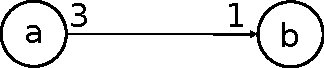
\includegraphics[scale=0.7]{capitoli/esplorazione-grafo-anonimo/imgs/n_28}
\end{center}

Se esco da $a$ su una porta diversa da 1 vado in stato $T$. Se trovo un valore
1, allora quell'arco è appartenente allo ST.

\begin{equation}
    f(T,i,d) =
    \left\{
    \begin{array}{r
            @{\quad{\mbox{se}}\quad}
            l}
        (N,1)   & i = d = 1                   \\
        (T,i+1) & i = 1 ~\textrm{e}~ d \neq 1 \\
        (B,i)   & i \neq 1                    \\
    \end{array}
    \right.
\end{equation}
\begin{itemize}
    \item Esco su porta 1 in stato \textit{Normal} se trovo che $v$ ha come
          grado 1 e la porta in cui entro su $v$ è proprio 1.
    \item Esco su porta $i+1$ ancora in stato \textit{Testing} se trovo ancora
          porta 1 nel nodo in cui vado ma il grado di questo nodo è diverso da
          1.
    \item Cambio in stato in \textit{Backtrack} e attraverso porta $i$ se
          trovo porta diversa da 1 sul nodo in cui sono andato.
\end{itemize}

\subsection{B: Backtrack}
\begin{center}
    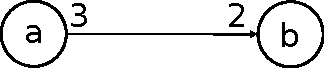
\includegraphics[scale=0.7]{capitoli/esplorazione-grafo-anonimo/imgs/n_28-2}
\end{center}

\begin{center}
    $f(B,i,d) = (N,1)$
\end{center}

\begin{itemize}
    \item Se mi posiziono su $v$ in stato di \textit{Backtrack} allora cambio
          stato in \textit{Normal} e attraverso porta 1, ovvero un arco che è
          sicuramente appartenente allo ST.
\end{itemize}

\subsection{Complessità}
\textbf{Perché è $\Pi(n) \leq 4n$ il costo?} Questo equivale a chiedersi quanto
vale il periodo $\Pi(n)$\\

L'automa deve esplorare in profondità tutto $T$ andata e ritorno, spendendo quindi
$2(n-1)$, a cui poi devo sommare i vari errori commessi dall'automa; può
commettere 1 errore su ogni nodo ma può sbagliare su tutti, quindi $n$.
Sbagliando deve anche tornare indietro, che è un altra aggiunta di $n$ errori.
Quindi si avrebbe in totale: $2(n-1)+n+n = O(4n) $ o anche $\leq 4n$. Se il
grafo è un \textbf{albero} siamo ottimi, poiché il lower bound è anch'esso
$n$.\\
In caso di \textbf{grafo completo} non posso esplorare l'albero convenientemente
a meno che non si parta dalla radice, in quel caso usando solo 2 stati si
avrebbe costo = $2n-2$. Potrei però costruire un grafo $G'$ ring, in quel caso
sempre con 2 stati si avrebbe un costo = $n$. Purtroppo l'idea del ring si può
applicare solo su grafi che siano Hemiltoniani (dotati di un cammino che tocca
tutti i nodi una e una sola volta), ma sapere se un grafo è Hemiltoniano è un
problema NP-completo.

Concludiamo quindi che il lower-bound è $2n-2$, esclusi i grafi Hemiltoniani.

\section{Prova formale della correttezza}
\begin{theorem}
    Sia $G$ un grafo di dimensione $n$ con orientamento locale
    compatibile con uno spanning-tree $T$. Se l'automa $A$ inizia da un qualunque nodo
    in un qualunque stato, dopo al più 2 step $A$ entra in un cammino chiuso $P$ e lo
    percorre per sempre. Inoltre $P$ è di lunghezza al più $4n-2$ e contiene tutti i
    nodi di $G$.
\end{theorem}
\begin{proof}\
    \begin{itemize}
        \item Sia $G$ un grafo con $n$ nodi;
        \item Sia $v$ un nodo arbitrario di $G$;
        \item Sia $e$ un arco dello ST di $v$ con porta 1.
    \end{itemize}
    Consideriamo ciò che otteniamo rimuovendo tale arco, il nostro T avrà allora 2
    sotto alberi, quello che contiene $v$ lo chiameremo $T_1$ e con $n_1$
    indichiamo il numero di nodi in $T_1$.

    Per dimostrare l'enunciato useremo la seguente proprietà:

    \paragraph{Claim:} Se $A$ entra in $v$ attraverso porta 1 in uno stato
    differente da \textit{Backtrack} allora prima o poi lascerà $v$ attraverso
    porta 1 nello stato \textit{Normal}. Inoltre, tra questi 2 eventi, esplora
    tutti i nodi di $T_1$ in al più $4n_1 - 2$ step, e non esce da nessun nodo
    non in $T_1$ attraverso porta 1 durante l'attraversamento.
    \begin{proof}
        Per poter provare il Claim ci si focalizza sul sottoalbero $T_v$ ottenuto
        tagliando l'arco con etichetta 1. Si prova quindi Per induzione sull'altezza
        di $T_n$:
        \begin{itemize}
            \item Base: $h(T_1) = 0 \Rightarrow v$ \textbf{è} una foglia in $T$.
                  \begin{itemize}
                      \item Se $v$ è una foglia anche su $G$, allora l'automa lascia
                            automaticamente la foglia $v$ attraverso porta 1 in
                            stato \textit{N} ed il claim è dimostrato. Questo avviene
                            perché $d=i$ quindi si va sullo stato \textit{N}.
                      \item Se invece il $d(v)>1$ su $G$, l'automa entra in $v$ in
                            testing $(T, i+1)$ ed attraverserà l'arco con
                            etichetta 2. $v$ è una foglia su $T$, e dato che $e$ è
                            in $T$, $e'$ non può esserlo, quindi la porta
                            nell'altro estremo non potrà mai essere 1. Quindi
                            tornerà indietro con \textit{B}. In questo caso avremo 2
                            step, derivati da $(4n_1 -2)$ con $n_1=1$
                  \end{itemize}
            \item Passo induttivo: $v$ \textbf{non} è una foglia in $T$.
                  \begin{itemize}
                      \item La porta "2" che è quella che l'automa attraverserà
                            una volta posizionato su $v$, ci conduce ad una
                            porta "1". Se andiamo a considerare il sotto albero
                            $T_2$ radicato in questo nodo avremo: $h(T_2) \leq
                                h(T_1) -1$, poiché si effettua uno step in
                            profondità dal nodo $v$ al sottoalbero ottenuto
                            tagliando l'arco con etichetta 1. Possiamo quindi
                            applicare l'ipotesi induttiva e avremo che in
                            $4n_2-2$ step verrà visitato $T_2$. Ora l'automa
                            torna in $v$ nello stato \textit{N}, la scelta che
                            seguirà dipende dal grado di $v$. Supponiamo $p$ la
                            label più grande di un albero radicato in $v$; in
                            generale avremo che per tutti gli archi con porta $i
                                \leq p$ l'automa esplorerà l'albero $T_i$ in al più
                            $4n_i - 2$ passi.\\
                            \textbf{Quanti passi in totale effettua
                                l'automa nei sotto alberi?}
                  \end{itemize}
        \end{itemize}
        \begin{equation*}
            \begin{split}
                \#Step & \leq \sum_{i=2}^{p} (4 n_i - 2 +2) +2= 4\sum_{i=2}^{p} (n_i)+2  = 4(n'-1)+2 = 4n'-2
            \end{split}
        \end{equation*}

        \begin{itemize}
            \item $(4 n_i - 2)$ Sono i passi per esplorare il singolo sotto
                  grafo.
            \item +2 dentro la parentesi sono i passi che l'automa fa verso il
                  sotto grafo per poi tornare al nodo di partenza.
            \item +2 fuori dalla parentesi sono i passi che l'automa fa qualora
                  ci fosse una porta che non conduce ad un sotto albero con
                  porta 1 dall'altra parte. L'errore lo fa a porta $p+1$,
                  infatti la sommatoria arriva fino a $p$.
            \item Dopo il primo $=$, $\sum_{i=2}^{p} (n_i)$ sono tutti i nodi
                  del sotto albero $T'$ tranne $v$, che sono infatti $(n'-1)$.
        \end{itemize}

        % \begin{comment}

        % %Questi sono i passi che fa l'automa in ogni sotto albero. A questi vanno
        % %aggiunti anche i passi per raggiungere i sotto alberi e esattamente 2 step
        % %qualora ci fosse un altro arco che non ha 1 nell'altra estremità.
        % \begin{equation}\nonumber
        %     \begin{split}
        %         \#passiTot & = \sum_{i=2}^{p} 4 n_i -2 + 2(P-1) + 2 = \\
        %         & 4 \sum_{i=2}^{p} n_i -2 - 2(P-1) + 2(P-1) + 2 =\\
        %         & 4 \sum_{i=2}^{p} n_i =  4(n'-1) +2 = 4n'-2
        %     \end{split}
        % \end{equation}


        % Dove:
        % \begin{itemize}
        %     \item $\sum_{i=2}^{p} n_i = (n'-1)$ fa quel valore perché sono tutti i
        %           nodi nei rispettivi sotto alberi, che vengono chiamati $n'$ -1 invece è
        %           perché la sommatoria inizia da 2 e quel -1 è esattamente il nodo $v$.
        %     \item La sommatoria indica tutti quelli che hanno porta 1 alla fine del
        %           link (nell'esempio sul quaderno erano $T_i, T_j, T_p$)
        %     \item $4n_i - 2$ Indica tutti quelli dentro al sottografo (numero di passi
        %           per attraversare tutti i nodi)
        %     \item $2(P-1)$ Tutti i passi da V ai sottografi (quelli tagliati) e
        %           viceversa. P indica tutti i vicini di V e -1 poiché è l'arco in entrata
        %           "dall'alto".
        %     \item +2 Se c'è qualche altro link oltre a P che non ha dall'altra parte
        %           etichetta 1, ed indica andare in Testing e tornare indietro con Backward.
        % \end{itemize}
        % \end{comment}

        Abbiamo quindi dimostrato il claim.
    \end{proof}

    \begin{proof}[Dimostrazione. \textbf{(Loop Infinito)}]\

        Andiamo a dimostrare ora che il ciclo in cui entra l'automa è infinito.
        Per come abbiamo definito l'etichettamento locale sappiamo che esisterà
        un arco con due "1" agli estremi e definiamo i nodi di questo arco come
        $V$ e $U$. In entrambi i sottoalberi radicati nei due nodi l'automa
        entrerà nello stato di \textit{Normal} su porta 1 e quindi è possibile
        applicare il \textbf{Claim}. Il numero dei passi sarà $4n' - 2$
        effettuati per esempio sul sottografo radicato in $V$, mentre $4n''-2$ nel
        sottografo radicato in $U$. Quindi:

        $$
            4n'-2 + 4n''-2 + 2 = 4n -2
        $$

        Dove il +2 indica l'andata e ritorno dall'arco
        con etichetta 1-1.\\
        Si avrà un ciclo infinito in cui vengono visitati tutti i nodi della
        rete in $4n -2$ passi.
    \end{proof}
    \begin{proof}[Dimostrazione. \textbf{(L'automa entra in $P$ in al più 2 archi)}]\

        L'automa inizia da uno stato e posizione qualsiasi; per definizione della
        funzione di transizione ci possono essere tre casi:
        \begin{itemize}
            \item Caso 1: L'automa lascia il nodo da porta 1 in stato
                  \textit{N}. Questo implica che l'automa entra immediatamente
                  nel ciclo infinito e chiuso $P$. [0 step]
            \item Caso 2: L'automa lascia il nodo in stato \textit{B}. In caso
                  di \textit{Backtrack}, per come abbiamo definito la
                  transazione dell'automa, il prossimo arco che si attraversa è
                  con porta 1 e si entra in stato \textit{N}, quindi siamo
                  dentro al ciclo $P$. [1 step]
            \item Caso 3: L'automa lascia il nodo $v$ attraverso l'arco $e$ di porta
                  $i$ con $i\geq2$ in stato \textit{T}. Abbiamo due possibilità:
                  \begin{enumerate}
                      \item L'arco $e$ è in $T$; implica che $e$ è già dentro il
                            cammino chiuso. [0 step]
                      \item L'arco $e$ non è in $T$; se così fosse all'altra
                            estremità non ci sarà sicuramente 1, quindi l'automa
                            arriva nell'altro nodo, cambia stato in \textit{B} e
                            ritorna nel nodo $v$ attraverso $e$ commettendo
                            esattamente due errori. Successivamente lascerà $v$
                            tramite porta 1 in stato \textit{N} poiché siamo in
                            stato \textit{B} ed entrerà nel ciclo infinito. [2
                                    step]
                  \end{enumerate}
        \end{itemize}
        Allora effettivamente in al più due step, che sono i due errori in $T$, si
        entra nel ciclo.
    \end{proof}
\end{proof}

\textbf{Voglio garantire la terminazione del protocollo: }
Per garantire la terminazione del protocollo si potrebbe controllare che esso
"passi" 3 volte sull'arco "eletto" (cioè quello che ha le due porte "1"), questo
si può fare arrivando ad avere 9 stati.

\section{Distributed Small Port}
Fino ad adesso abbiamo supposto che lo Spanning Tree venisse dato in input,
proviamo a costruirlo dato un generico Grafo. Andiamo ora a vedere un altro
algoritmo che ci permetterà di costruire uno ST con orientamento locale. Questo
è chiamato \texttt{Distributed Small Ports} (\texttt{DSP}) e si basa su
\texttt{Shout+}.
\begin{itemize}
    \item Solamente il nodo con l'automa sopra è sveglio e sarà la radice $r$
          dell'albero.
    \item La radice invia un messaggio $Q$ a tutti i suoi vicini.
    \item Un qualsiasi nodo $v \neq r$ è sveglio quando gli arriva almeno un
          messaggio. Questo sceglie come padre il nodo che gli ha inviato per
          primo un messaggio.
          \begin{itemize}
              \item Ogni nodo sveglio invierà una domanda $Q$ (sei un mio vicino
                    nello ST?) ed aspetta una risposta \texttt{SI}/\texttt{NO}.
              \item Quando un nodo invia un \texttt{SI}, mette $1$ sulla porta
                    sull'arco utilizzato, perché questo conduce verso la radice.
              \item Quando il nodo $r$ (radice) riceve un \texttt{SI}, ordina i
                    \texttt{SI} da $1$ a $|F_v|$, e le restanti risposte li
                    ordina da $|F_v|+1$ a $d_v$.
              \item Quando un nodo $v \neq r$ riceve un ``\texttt{SI}'' assegna
                    i numeri di porta da 2 al $|F_v|$. Infine assegna i
                    rimanenti numeri di porta agli archi rimanenti.
          \end{itemize}
\end{itemize}

%Finalmente $v$ manda un messaggio di "Parent" a tutti i suoi vicini scelti come
%parenti ed un messaggio di "Hello" a tutti quelli rimanenti. Quando un nodo $u$
%riceve un messaggio da tutti i suoi vicini, sceglie l'orientamento locale come
%segue: \begin{itemize} Sia p il numero di messaggi "Parent" che un nodo $u$ ha
%ricevuto: \item Se $u$ è la radice, allora assegna arbitrariamente i numeri di
%porta da 1 a $p$ agli archi $p$ che conducono ai mittenti di messaggi "Parent".
%Assegna poi i rimanenti numeri di porta ai rimanenti archi, se presenti. \item
%Se $u$ non è la radice, assegna i numeri di porta da 1 al numero di vicini
%scelti come Parent. Poi assegna numeri di porta da 2 a $p+1$ al $p$-esimo arco
%che porta al mittende di un messaggio "Parent", se presenti. Infine assegna i
%rimanenti numeri di porta agli archi rimanenti. \end{itemize}
Ogni nodo sveglio invierà una domanda $Q$: ``Sei un mio figlio nello ST?'' ed
aspetta la risposta \texttt{SI}/\texttt{NO}. Possiamo eliminare i messaggi
\texttt{NO}, desumendoli dalla ricezione di una domanda.


\begin{center}
    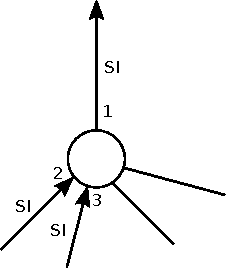
\includegraphics[scale=0.75]{capitoli/esplorazione-grafo-anonimo/imgs/n_32}
\end{center}

\begin{theorem}
    L'algoritmo \texttt{DSP} costruisce uno ST del grafo e crea un
    orientamento locale compatibile con lo stesso, utilizzando $M[$\texttt{DSP}$/
                RI] = 2m$. [Non fatto a lezione]
\end{theorem}

Si adatta a reti dinamiche:
\begin{itemize}
    \item se appare un arco nuovo, non lo consideriamo nell'esplorazione:
          \begin{center}
              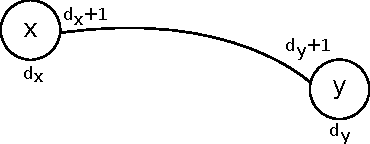
\includegraphics[scale=0.75]{capitoli/esplorazione-grafo-anonimo/imgs/n_33}
          \end{center}
    \item se appare un nuovo nodo con dei nuovi archi, scelgo un arco e metto
          \#porta 1 nell'arco che conduce al padre, mentre nel nodo raggiunto devo
          ``riaggiustare'' le numerazioni.
          \begin{center}
              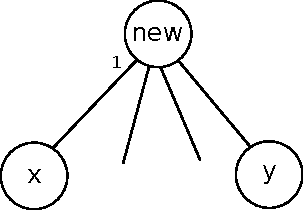
\includegraphics[scale=0.75]{capitoli/esplorazione-grafo-anonimo/imgs/n_34}
          \end{center}
    \item cancellazione di un arco non in ST: devo compattare i numeri di porta;
    \item cancellazione di un arco nello ST: devo sostituire integralmente lo ST;
    \item se cancelliamo un nodo di grado 1 (foglia nello ST) basta rinumerare:
          \begin{center}
              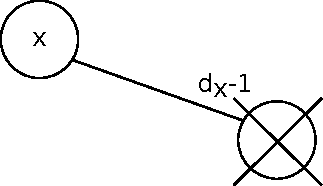
\includegraphics[scale=0.75]{capitoli/esplorazione-grafo-anonimo/imgs/n_35}
          \end{center}
    \item se cancelliamo un nodo di grado $> 1$, dobbiamo ricostruire lo ST.
\end{itemize}

\section{Miglioramento del Bound di 4n: Ci si basa sul numero di etichetta inserito}

\emph{Fast Periodic Graph Exploration
    with Constant Memory, L. Gasieniec, R. Klasing, R. Martin, A. Navarra, X.
    Zhang}\\

Si può fare di meglio? Si!\\ \textbf{Facciamo in modo che all'etichetta più
    bassa corrisponde il sottoalbero più alto.} In pratica l'automa avendo una
"memoria" del passo precedente conosce la massima altezza che dovrà percorrere
nell'arco successivo. \textbf{Si ordinano le etichette di un generico nodo V in
    maniera inversamente proporzionale alla dimensione dei suoi sottoalberi.}
Ovvero, più è piccola l'etichetta e maggiore sarà l'altezza del sotto albero. Le
foglie quindi avranno tutte la stessa etichetta, quindi l'automa sbaglia nella
prima o poi non sbaglia più. Questo funziona anche con le altre strutture della
stessa altezza, dato che avranno lo stesso numero di porta, l'automa sbaglia una
volta e poi finché il numero di porta resta quello non sbaglia più.

\subsection{Descrizione delle strutture possibili}
Avendo questo ordinamento, la struttura più piccola che può stare nel
sottoalbero è una foglia, che quindi avrà etichetta più grande di tutte le
altre. Le foglie quindi avranno etichettamento consecutivo e quindi è possibile
sbagliare nel primo arco, ma successivamente l'automa saprà che da li in poi
saranno tutte foglie, e quindi non sbaglia più. Questo metodo si applica anche
qualora ci fossero più strutture con la stessa etichetta, poiché potrò sempre
risparmiare errori una volta aver sbagliato nella prima. Elenchiamone alcune:\\
Struttura prima di trovare una foglia: Un albero con altezza uno, ovvero due
nodi messi a fila.\\
Ora abbiamo due possibilità:
\begin{itemize}
    \item Due nodi messi in fila
    \item Un nodo con due foglie.
\end{itemize}
Per ridurre il $4n$ dovrei eliminare un quantità di errori lineare rispetto al
numero di nodi.
\subsection{Protocollo costruzione albero}

\begin{lstlisting}

Procedure Color(node v)
	node v become RED
	all nodes at distance 1 from v become GREEN
	all not yet colored nodes at distance 2 from v become BLUE
	
Procedure Backbone-Construction(G) -> Tree
	pick an arbitrary node $v \in V$
	Color(v)
	$V_B = \{ v \}$ //nodi della backbone (all'inizio solo v)
	$E_B = \{ \emptyset \}$ //archi della backbone (all'inizio nessuno)
	while (the set of not colored nodes in $G \neq \emptyset$)
		pick a not colored node at distance 1 from some BLUE node $w_1$ 
			which is itself connected via node $w_2$ to some RED node v
		Color(v)
		$V_B = V_B \cup \{ w_1, w_2, v \}$
		$E_B = E_B \cup \{ (v',w_2), (w_2, w_1), (w_1, v)\}$
		node $w_1$ and $w_2$ becomes YELLOW
		
Procedure Tree-Construction (G, B /*Backbone di G*/) -> ST
	$V_T = V_B$
	$E_T = E_B$
	
	[Stiamo estendendo la backbone in maniera tale da prendere i nodi a distanza
    1 dai rossi. In termini di errori troviamo dei vantaggi poiche cosi
	facendo, i nodi rossi hanno il grado all'interno dell'albero uguale a
    quello che hanno nel grafo. Se il robot quindi si deve muovere da un nodo
    rosso non puo' sbagliare, dato che tutti 
    gli archi di un nodo rosso sono tutti appartenenti allo
    ST che stiamo costruendo.]
	
	foreach node $v \in V\diagdown V_T$ at distance 1 from a RED node $v' \in V_B$ do
		$V_T = V_T \cup \{v\}$
		$E_T = E_T \cup \{(v,v')\}$
	foreach node $v \in V\diagdown V_T$ at distance 1 from some node $v' \in V_T$ do
		$V_T = V_T \cup \{v\}$
		$E_T = E_T \cup \{(v,v')\}$ 
		[Tutti i nodi che sono rimasti fuori dall'albero sono a distanza 1 da questo, e quindi li prendo]
    each YELLOW node v not connected to any BLUE made v' by edge $(v,v')\in E_T$ becomes ORANGE
\end{lstlisting}

\paragraph{Osservazioni:}
%\vspace{-10mm}
\begin{itemize}
    \item I nodi rossi hanno tutti gli archi incidenti dentro lo ST.
    \item Non è possibile che ci sia un nodo verde a distanza 1 da due nodi rossi.
    \item Se prendiamo un qualunque nodo dell'albero che non sta nella backbone la
          sua distanza massima sarà 2, proprio per come è stato costruito
    \item non si può comunque avere sottoalberi con altezza maggiore di 2
\end{itemize}

La Backbone è formata da nodi Rossi e Gialli con la proprietà che se il percorso
che connette due nodi rossi contiene solo nodi gialli, allora ne contiene
esattamente due di questi. I nodi rimanenti sono colorati o di Verde o di Blu se
la loro distanza da un nodo rosso è 1 o 2 rispettivamente. La procedura ricolora
tutti i nodi Gialli, che non hanno nodi Blu come vicini, in nodi Arancioni.
Questa colorazione sarà utile per calcolare la lunghezza della distanza $P$.

Per andare ad etichettare il grafo dell'esempio sul quaderno le etichette 1 si
mettono su tutti gli archi per andare VERSO la radice (dalle 4 regole viste
all'inizio del paragrafo). I numeri di porta restanti vanno messi in base al
numero di nodi nel sottoalbero e bisogna comunque numerare gli archi che non
appartengono allo ST.

\textbf{Quanto risparmiamo con questo metodo?}\\
Se consideriamo un nodo rosso, esso avrà un certo numero di connessioni della
backbone, se ora consideriamo il resto del vicinato e lo ordiniamo in ordine
decrescente di size dei sottoalberi, più a destra possibile si avranno le foglie
(gruppo L nel disegno), poi avremo le cosiddette foglie estese (gruppo E), poi i
generici sottoalberi (gruppo A)

\begin{center}
    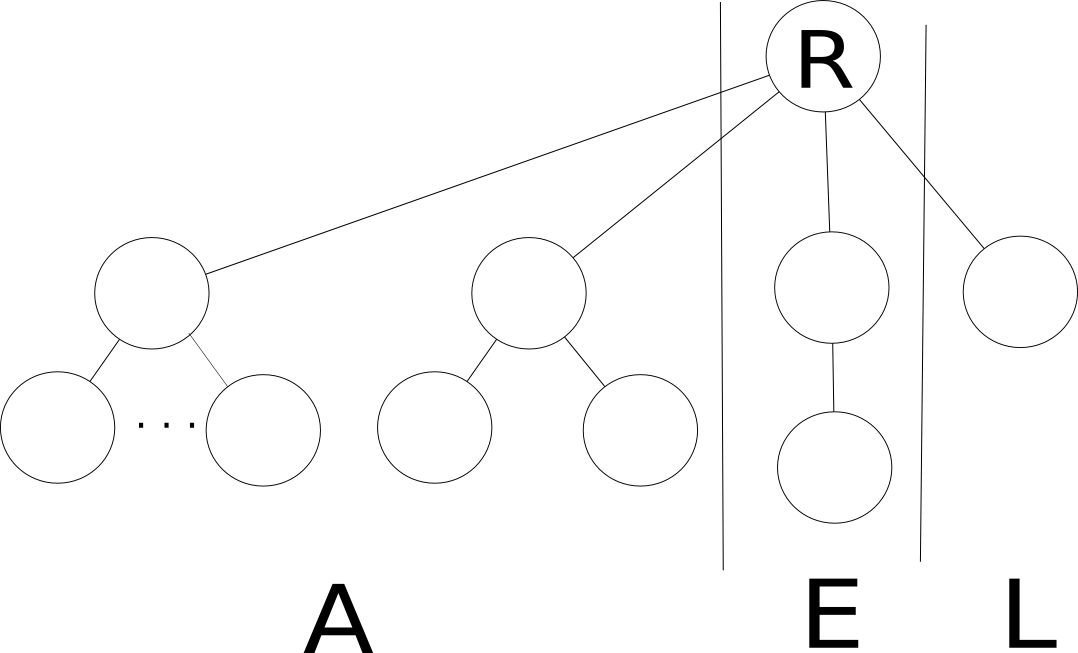
\includegraphics[scale=0.15]{capitoli/esplorazione-grafo-anonimo/imgs/automa1.png}
\end{center}

Consideriamo le tre tipologie in maniera separata, nel gruppo L l'automa farà al
massimo un errore, nel gruppo E ne farà al massimo 2, uno nella foglia e uno nel
nodo intermedio per controllare se ha un altro figlio, cioè se è ancora nel caso
A, mentre per il tipo A saranno 2 errori per ogni tipo di sotto albero.\\ L'idea
principale del protocollo è che inseriamo questi numeri di porta per fare in
modo che \textbf{il robot esplori prima i sotto alberi più grandi e poi quelli
    più piccoli a mano a mano.}

$v$ è un nodo rosso, indichiamo ad esempio $S_L(v)$ (numero di nodi di tipo $L$ del
nodo $v$) :
\begin{equation*}
    S_L(v) = \begin{cases} 0, & \mbox{se il numero di figli di v di tipo L è 0} \\
              1, & \mbox{altrimenti}\end{cases}
\end{equation*}
\begin{equation*}
    S_E(v) = \begin{cases} 0, & \mbox{se il numero di figli di v di tipo E è 0} \\
              1, & \mbox{altrimenti}\end{cases}
\end{equation*}
\begin{equation*}
    S_A(v) = \#figliDiTipo A
\end{equation*}

\begin{equation}
    \begin{array}{ccc}
        S_L = \sum_{v \in RED} s_L(v) &
        S_E = \sum_{v \in RED} s_E(v) &
        S_A = \sum_{v \in RED} s_A(v)   \\
        S_Y = \#nodiGialli            &
        S_O = \#nodiArancioni         &
        S_R = \#nodiRossi
    \end{array}
\end{equation}
Sia $n$ il numero di nodi e $p$ il numero di errori che possono commettere.
\paragraph{Calcolo di n}\ \\
Avremmo: $n \geq 3 S_A + 2 S_E + S_L + S_O + 2 S_Y + S_R$\\
Poiché 3 sono il numero di nodi che creano un sottoalbero di tipo A, 2 $S_e$
indica il numero di nodi se l'albero è una foglia estesa e 2 $S_y$ poiché i nodi
gialli sono al più 2??? I nodi yellow che non sono diventati Orange è perché
hanno dei vicini Blue.
\paragraph{Calcolo della Penalty [Vedere quaderno per i disegni su dove commetto
            errori]:}\ \\
Quanti errori commetto nella struttura $S_A$? Al più due.\\
Quanti errori commetto nella struttura $S_E$? Al più due.\\
Quanti errori commetto nelle foglie? Solo uno.\\
Quanti errori commetto sui nodi gialli? Al più due\\
Quanti errori commetto sui nodi Orange? Solo uno.\\
Quindi possiamo concludere che: la penalty è : \\
$p \leq 2 S_A + 2 S_E + S_L + S_O + 2 S_Y$\\
Mettiamoli in corrispondenza: \\
$p \leq 2 S_A + 2 S_E + S_L + S_O + 2 S_Y$\\
$n \geq 3 S_A + 2 S_E + S_L + S_O + 2 S_Y + S_R$\\

Sfruttiamo le seguenti proprietà per stimare il rapporto $p/n$
\begin{itemize}
    \item $S_Y + S_O = 2 S_R - 2$ Poiché $S_Y + S_O$ sono intermedi ai nodi rossi,
          se li sommo tutti ottengo due volte il numero dei rossi. (vedere quaderno per
          disegno)
    \item $S_E \leq S_R$, $S_L \leq S_R$
    \item $S_A \geq 0$
\end{itemize}
sommando sopra e sotto $S_O$ avremo: \\
$$\frac{2 S_A + 2 S_E + S_L + 2(S_Y + S_O)}{3 S_A + 2 S_E + S_L + 2(S_O + S_Y) +
        S_R} < \frac{2 S_A + 2 S_E + S_L + 4 S_R}{3 S_A + 2 S_E + S_L + 5 S_R} \leq
    \frac{2 S_A + 7 S_R}{3 S_A + 8 S_R} $$

Vediamo quindi il costo di questo algoritmo:\\
$$ 2n - 2 + 2p < 2n -2 + 2 \frac{7}{8} n = 3.75n -2 $$ Si ha 2P poiché commetto
l'errore e torno indietro.\\
Risposta : SI, si può fare di meglio.\\

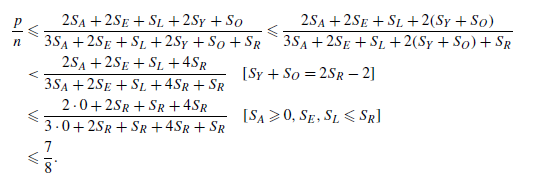
\includegraphics[]{capitoli/esplorazione-grafo-anonimo/imgs/66.png}\\
\textbf{Osservazione}: Senza stati, quindi senza memoria, il bound corrente è
4n-2.\\
$$O(2.8n) \leq Senza memoria (senza stati) \leq 4n-2$$
$$2n-2 \leq Con memoria \leq 3.5n -2 $$

